% Public explainer for llm-nav-shield, written for a non-specialist reader.
% Every number and every quoted proposal is taken from the committed
% records in this repository; the figures are the ones regenerated by
% tools/render_figures.py from the evaluation's own dumps.
%
% Build from this directory:  latexmk -pdf explainer.tex
%
% When the evaluation changes, the counts in "What the model actually
% proposed" and "The cell that must be zero" must be re-checked against
% reports/results/shield_eval_summary.txt. They are prose, so nothing
% enforces them.
\documentclass[11pt,a4paper]{article}

\usepackage[margin=2.4cm,top=2.2cm,bottom=2.2cm]{geometry}
\usepackage[T1]{fontenc}
\usepackage[utf8]{inputenc}
\usepackage{lmodern}
\usepackage{microtype}
\usepackage{graphicx}
\usepackage{xcolor}
\usepackage{titlesec}
\usepackage{enumitem}
\usepackage[hidelinks]{hyperref}
\usepackage{fancyhdr}
\usepackage{tcolorbox}
\tcbuselibrary{skins,breakable}

\graphicspath{{../figures/}}

\definecolor{navy}{HTML}{0F2F52}
\definecolor{gold}{HTML}{B08D3F}
\definecolor{ink}{HTML}{1A1A1A}
\definecolor{soft}{HTML}{F7F5F0}
\definecolor{rule}{HTML}{D8D3C8}

\color{ink}
\linespread{1.09}
\setlength{\parskip}{6pt}
\setlength{\parindent}{0pt}

\titleformat{\section}{\large\bfseries\color{navy}}{}{0pt}{}
\titlespacing*{\section}{0pt}{16pt}{6pt}

\pagestyle{fancy}
\fancyhf{}
\renewcommand{\headrulewidth}{0pt}
\fancyfoot[C]{\small\color{gray}\thepage}

\newtcolorbox{quotebox}[1][]{
  enhanced, breakable, colback=soft, colframe=gold,
  boxrule=0pt, leftrule=2.5pt, arc=0pt, outer arc=0pt,
  left=10pt, right=10pt, top=8pt, bottom=8pt, #1}

\newcommand{\code}[1]{{\ttfamily\small #1}}

\begin{document}

\begin{center}
{\LARGE\bfseries\color{navy} Wrong, or impossible?}\\[6pt]
{\large What a robot should do when its AI hands it a bad route}\\[12pt]
{\small Munawar Kazmi \;\textbullet\; \href{https://munawarkazmi.com}{munawarkazmi.com}}\\[2pt]
{\small A plain-language guide to \textbf{llm-nav-shield}, an open safety layer between language models and robot navigation.}\\[2pt]
{\small Code, data, and every figure: \href{https://github.com/munawarkazmi/llm-nav-shield}{github.com/munawarkazmi/llm-nav-shield}}
\end{center}

\vspace{4pt}
{\color{rule}\hrule height 1pt}
\vspace{10pt}

\section{A robot, a map, and a confident suggestion}

Suppose you want a small indoor robot to cross an office. You hand the problem to a language model: here is a map of the building, here is where you are, here is where you need to be, give me a route.

The model answers immediately and fluently. A neat list of coordinates, start to finish. It looks like a route. It is formatted like a route.

Now: do you drive the robot along it?

This document is about what has to sit between that answer and the wheels. It is a working system, and the numbers in it come from replaying forty real routes that a real model produced.

\section{Checking is not enough}

The obvious first answer is: check the route before running it. That is correct and it is not sufficient, for a reason that becomes obvious the moment you try it.

Checking tells you the route is bad. It does not tell you what to do next. And ``bad'' turns out to hide two completely different situations that demand opposite responses:

\begin{itemize}[leftmargin=1.4em,itemsep=2pt]
\item \textbf{The model was wrong, and a good route exists.} Here the right response is to throw away the model's answer and use the good route instead. The robot still does the job.
\item \textbf{There is no safe route at all.} The goal is walled off, or every approach is blocked. Here the right response is to stop and say so. Any system that produces an answer anyway is inventing one.
\end{itemize}

A system that cannot tell those apart is not a safety system. If it always produces a route, it will confidently produce one for the sealed room too.

\begin{quotebox}
The distinction this project is built around: ``the model was wrong, here is the correct path'' versus ``there is no safe action, stop.'' Safe autonomy needs both, and needs to know which is which.
\end{quotebox}

\section{What was built}

llm-nav-shield sits between the language model and the robot. Every proposed route goes through the same gate, and lands in exactly one of five outcomes:

\begin{itemize}[leftmargin=1.4em,itemsep=2pt]
\item \textbf{Forwarded} unchanged, if the model's route is both safe and actually ends at the goal.
\item \textbf{Recovered from unsafe}, if the route would hit something: a classical planner computes a provably correct route instead, which is then re-checked before anything moves.
\item \textbf{Recovered from off-goal}, if the route is perfectly safe but does not go where it was asked to go.
\item \textbf{Halted}, if no safe route exists at all.
\item \textbf{Fallback unsafe}, if the replacement route itself failed the checks. This one must never happen, and the automated tests fail the build if it ever does.
\end{itemize}

Two details matter more than they look. First, those five outcomes were written down and committed to the repository \emph{before} any results were published, so there is no possibility of inventing a flattering category after seeing the data. Second, the word ``shield'' is not decoration: it follows established usage from safety research, where a shield is a component that sits in front of a learned system and enforces what it is allowed to do.

The two things doing the actual work are not new either, and that is deliberate. The safety checker and the classical planner are separate, previously verified projects, pulled in at exact versions. The planner has been checked against a reference implementation across 185,237 randomly generated replanning problems. This repository is the composition: the wiring, the decision gate, and the evidence that the combination behaves.

\section{What the model actually proposed}

Forty scenarios. One model, qwen2.5 7B, with randomness turned off so the results are reproducible. Every one of its forty answers is committed to the repository, along with the exact map it was looking at.

Of those forty routes, \textbf{two} were both safe and actually arrived at the goal.

The other thirty-eight failed, and the ways they failed are worth naming, because they are not subtle:

\begin{itemize}[leftmargin=1.4em,itemsep=2pt]
\item \textbf{Teleporting} (18 routes). Consecutive waypoints too far apart for a robot to travel between. The route is only physically possible if the robot can jump.
\item \textbf{Leaving the map} (9 routes). Waypoints outside the mapped area entirely, into space the robot has never seen and was told not to enter.
\item \textbf{Driving through walls} (8 routes). Waypoints on the far side of an obstacle, with the path between them passing straight through it.
\end{itemize}

Separately from safety, 18 of the 40 routes did not respect the requested start and end points at all.

None of this means the model is useless or stupid. It means an unchecked language model is not a source of routes you can drive a robot along, which is precisely the assumption a safety layer exists to remove.

\section{The proposal that changed the design}

Before publishing any results, a dry run turned up one case that quietly broke the whole idea.

Here is what the model proposed for scenario 9, in full. This is the entire route:

\begin{quotebox}
\code{[[0.475, 6.525], [0.975, 6.525], [0.975, 6.725]]}
\end{quotebox}

Three points. The robot moves half a metre to the right, then twenty centimetres up, and stops. Total distance travelled: 0.7 metres.

The goal was 4.8 metres away.

Every step of that route is perfectly safe. It hits nothing, it leaves nothing, it teleports nowhere. A safety checker, asked ``is this route safe?'', correctly answers yes. And a system that only asked about safety would have handed this to the robot and reported success.

That is a safe plan to the wrong place: a mission failure wearing a safety pass. The gate was changed, before any results existed, to require both properties. A route is forwarded only if it is safe \emph{and} it ends where it was asked to end. Three of the forty proposals turned out to be exactly this shape.

\begin{quotebox}
Safety and doing the job are separate questions. Scoring only one of them lets a robot that does nothing look like a robot that does everything right.
\end{quotebox}

\section{Recovering: the model was wrong, here is the route}

When a proposal fails, the shield does not simply refuse. It sends the same start and goal to the classical planner, which computes a route on a fine-grained version of the map and is guaranteed to find the shortest safe one if any exists.

That recovered route is then checked twice more before anything moves: once by the same safety checker, and once by a second pass over the same rule sampling four times more finely. The second pass guards against a coarse sample stepping over a thin obstacle. It is not an independent opinion, because it shares the first one's model of the robot, and on this data the two have never disagreed. The route is also checked for actually reaching the goal.

\begin{figure}[t]
\centering
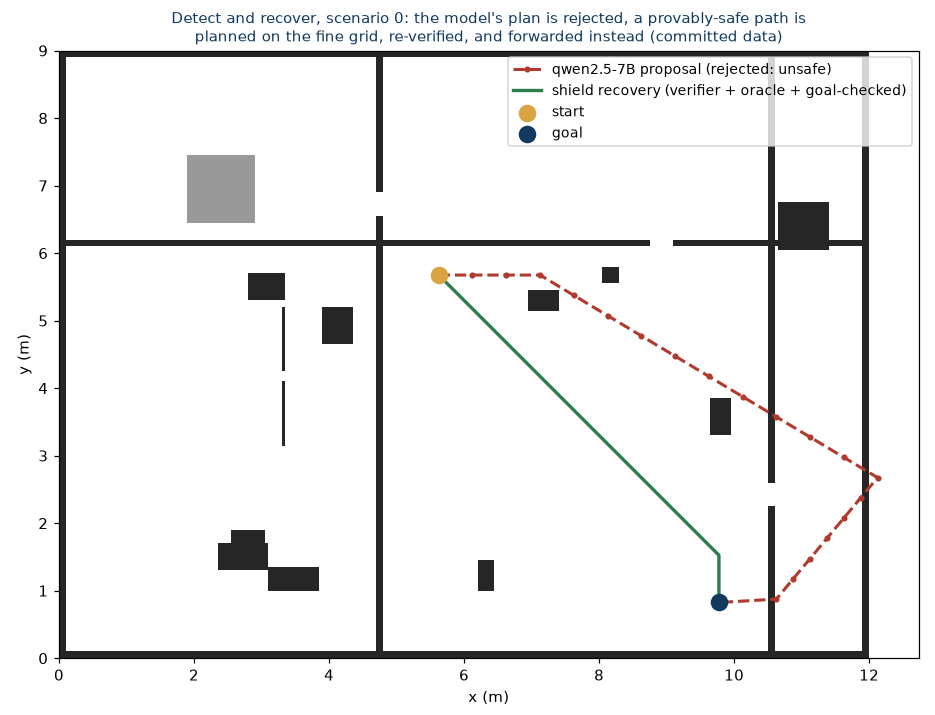
\includegraphics[width=\linewidth]{shield_recovery.png}
\caption{\small A real case from the committed data. The dashed red line is the model's proposal, which the checker rejected. The solid green line is the route the shield planned instead, re-verified twice and confirmed to reach the goal. Black shapes are walls and furniture.}
\end{figure}

All thirty-eight failed proposals were recovered this way. Every replacement route passed both checkers and the goal check. The count of unsafe replacement routes was zero, and the automated tests fail the build if it is ever anything else.

The entire decision, checking the proposal, planning a replacement, and checking that twice, takes a median of half a millisecond.

\section{Halting: there is no safe action, stop}

The forty original scenarios all have reachable goals, so none of them can test the branch that matters most. A safety system that has never had to say ``no'' has not been tested, it has been demonstrated.

So a second suite was built by taking the first ten scenarios and walling the goal off completely, leaving no safe route to it at all. In every one of those ten, the only correct behaviour is to halt.

\begin{figure}[t]
\centering
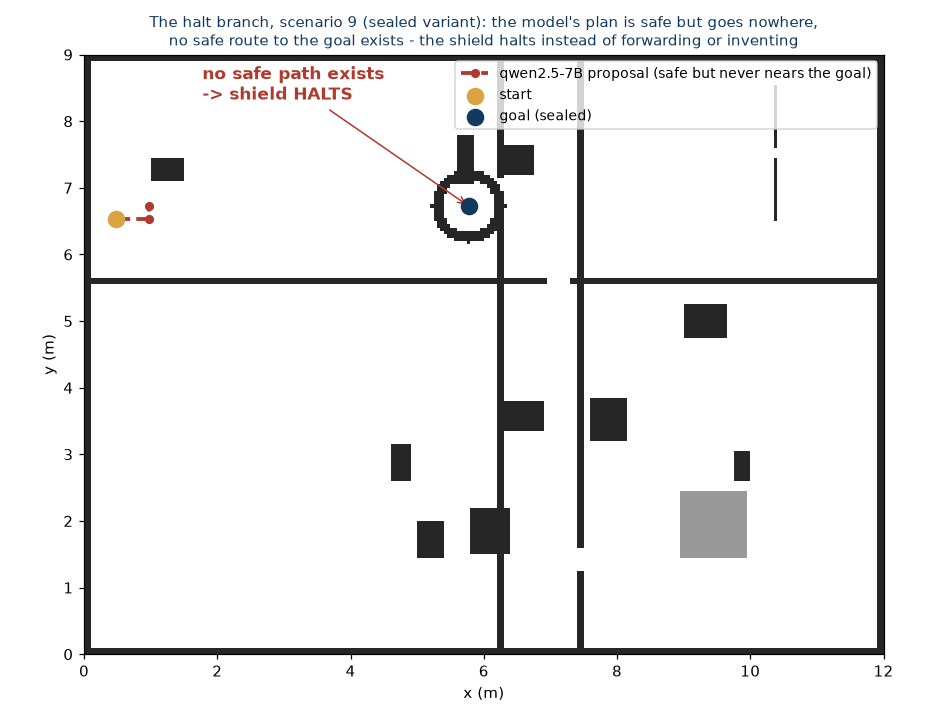
\includegraphics[width=\linewidth]{shield_halt.png}
\caption{\small The same scenario 9, with the goal now sealed behind walls. The model's proposal is still safe and still goes nowhere. No safe route to the goal exists, so the shield halts rather than forwarding the useless route or inventing a plausible one.}
\end{figure}

The shield halted in all ten. It did not forward the model's route, and it did not produce a route of its own. Both of those would fail the automated tests.

This is a small number and a constructed one, and it is stated that way. But the branch exists, it is exercised, and its correctness is asserted on every change to the code.

\section{The cell that must be zero}

Every one of the five outcomes is counted, and the counts are printed by a single command that anyone can run. One of those counts is load-bearing: the number of times a replacement route was itself unsafe or missed the goal. It is zero, and the continuous integration system rejects any change that makes it anything else.

That is the difference between a system that reports how well it did and a system that cannot be merged if it did badly. The claim is not ``we tested it and it worked''. The claim is ``it cannot be changed in a way that breaks this without the change being refused''.

Reproducing all of it requires no AI model, no graphics card, and no internet access. The forty model responses are committed, so the evaluation replays them deterministically on any computer, and the automated tests do exactly that on every change.

\section{What this does not show}

One model, at one setting, on forty scenarios, plus ten halt cases built by hand. All of it in simulation: no physical robot was involved at any point. The claims here are about this system's behaviour on this committed data, not about language models in general, and the timing figure depends on the machine it runs on while the counts do not.

The obvious next step is real hardware, and the honest statement is that it has not happened yet.

\section{Why it matters}

Language models are being connected to things that move. The interesting question is not whether they are sometimes wrong, because they obviously are. The question is what the surrounding system does about it, and whether it can tell the difference between a fixable mistake and a situation with no safe answer.

Detect, recover, or halt. Three outcomes, chosen mechanically, with the dangerous one ruled out by a test that fails the build.

\vspace{6pt}
{\color{rule}\hrule height 1pt}
\vspace{6pt}

{\small Every route, every map, every figure, and the code that scores them are public. This guide is part of a wider line of work: a benchmark measuring \emph{how} language model planners fail, a verifier that detects those failures, a planner that produces provably correct alternatives, and this repository, which composes them.\\
Repository: \href{https://github.com/munawarkazmi/llm-nav-shield}{github.com/munawarkazmi/llm-nav-shield}}

\end{document}
